\section{Аналитический раздел}

%В этом разделе будет приведен анализ предметной области в сфере организации футбольных турниров, приведена постановка задачи и формализация данных.
%Также будут описаны системные польвозатели.

\subsection{Анализ предметной области}

Футбольный турнир --- это соревнование, в котором несколько команд сражаются между собой, чтобы определить лучшую из них \cite{raytracin}.

Основная задача футбольного турнира заключается в создании среды для соревнования между командами с целью определения победителя и награждения его призом или званием чемпиона.

Турниры по футболу обычно проводятся в формате сезона, который на протяжении определенного периода времени, например, нескольких месяцев или года.

Основными правилами турнира по футболу являются:
\begin{enumerate}
	\item Турнир может проводиться по круговой форме (каждая команда играет со всеми остальными командами один или два раза).
	\item На групповом этапе команды ранжируются на основе очков, полученных в матчах (победы дают 3 очка, ничьи --- 1 очко, поражения не дают очков).
	\item Если две или более команды имеют одинаковое количество очков, для определения рейтинга будут использоваться второстепенные критерии, такие как разница мячей, количество забитых голов или результаты прямых матчей.
	\item Оргкомитет спланирует и объявит график соревнований до начала турнира. Этот календарь включает время и место проведения матчей и может быть скорректирован при необходимости по таким причинам, как плохая погода или проблемы безопасности.
\end{enumerate}
\subsection{Постановка задачи}
Разработка удобной платформы для футбольных сообществ, позволяя создавать и управлять тунирами с минимальными усилями. Там пользователи могут легко создавать турнир, состовлять расписание матчей, вводить результаты...
Необходимо создать приложение, чтобы упростить процесс управления футбольнами турнирами.

На рисунке \ref{img:A0} приведены IDEF0-схемы для поставленной задачи.
\begin{figure}[h]
	\centering
	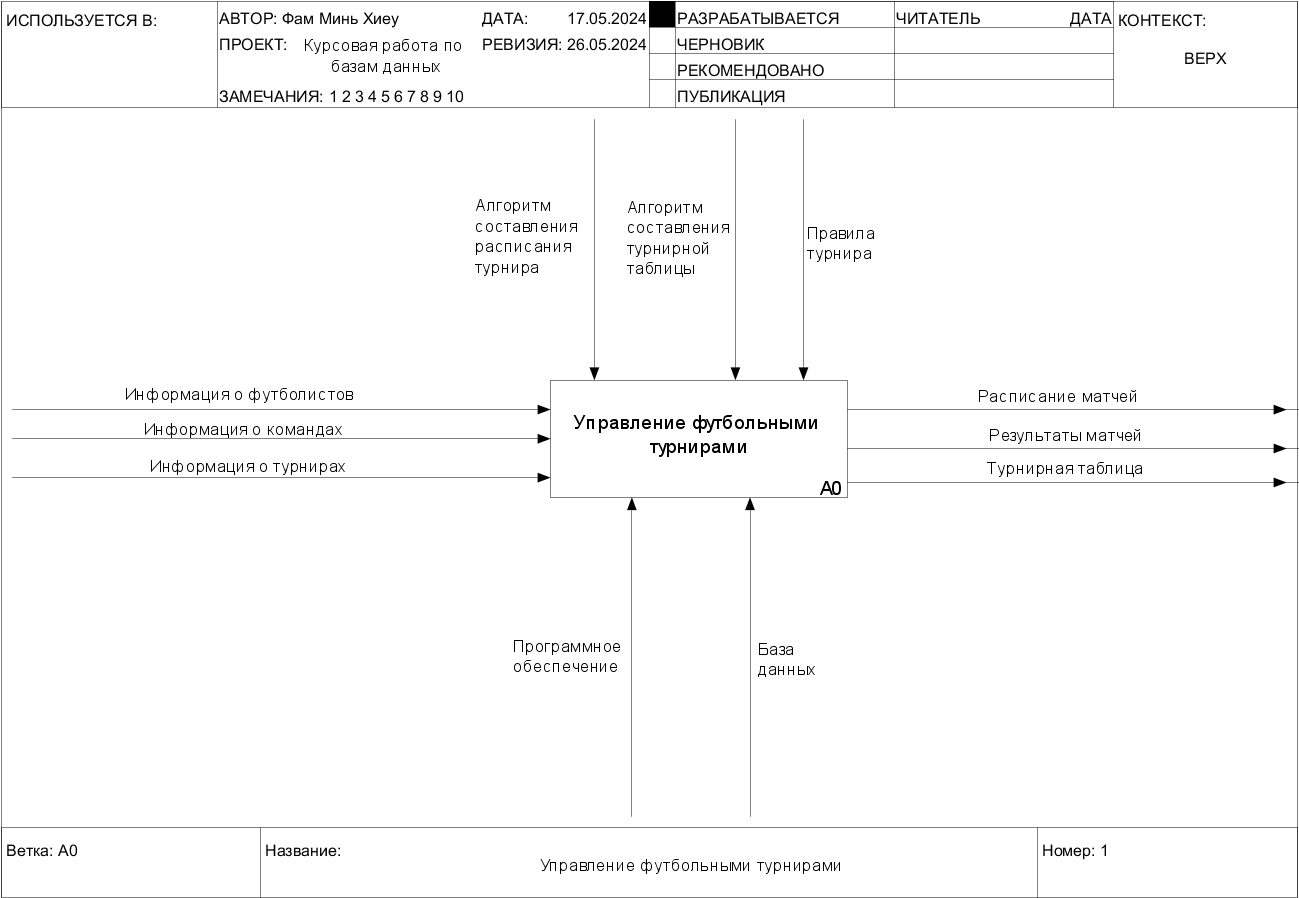
\includegraphics[height=0.45\textheight]{img/idef0/01_A0.png}
	\caption{Контекстная диаграмма (A-0)}
	\label{img:A0}
\end{figure}

%\begin{figure}[h]
%	\centering
%	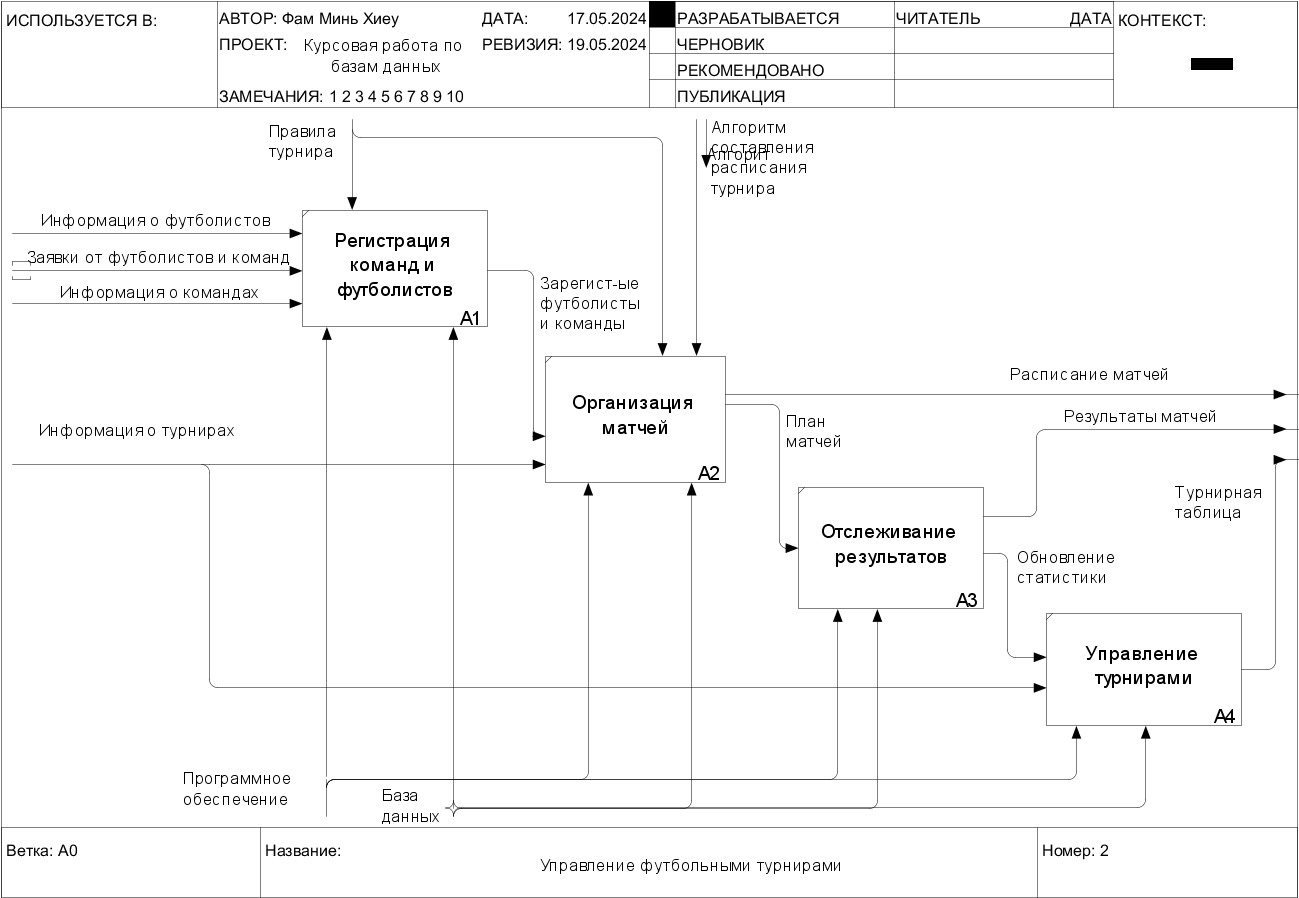
\includegraphics[height=0.45\textheight]{img/idef0/02_A0.png}
%	\caption{Декомпозиция контекстной диаграммы}
%	\label{img:A1}
%\end{figure}
\subsection{Анализ баз данных по модели данных}
Модель данных --- совокупность правил порождения структур данных в базе данных, операций над ними, а также ограничений целостности, определяющих допустимые связи и значения данных, последовательность их изменений \cite{roders}.

По модели баз данных рассматривается три основных типа:
\begin{enumerate}
	\item Дореляционные.
	\item Реляционные.
	\item Постреляционные.
\end{enumerate}
\subsubsection{Дореляционные}
Иерархическая и сетевая модели баз данных входят в категорию дореляционных моделей данных.
Иерархическая модель организует данные в виде дерева с отношениями предок-потомок.

На рисунке \ref{img:hierachy} приведена схема иерархической модели.

\begin{figure}[h]
	\centering
	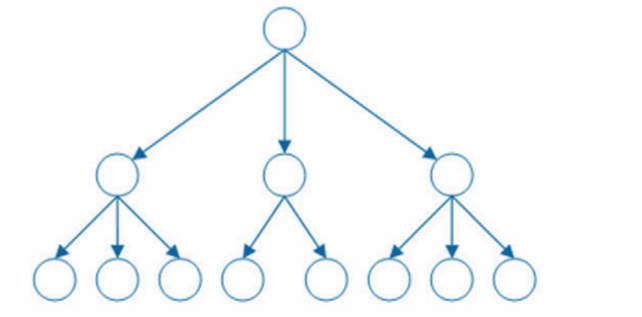
\includegraphics[height=0.25\textheight]{img/hierachy.png}
	\caption{Cхема иерархической модели \cite{roders}}
	\label{img:hierachy}
\end{figure}

Эта модель подразумевает, что каждая запись имеет одного родителя и несколько детей.
Связи между записями реализуются через физические указатели.
Недостатком является невозможность реализации отношений многие ко многим и ситуаций, когда у записи несколько предков.

Сетевая модель организует данные в виде графа, в которой у дочерней записи может быть несколько родителей.
Она отличается от иерархической модели тем, что разрешает такие множественные связи.
Основным недостатком сетевой модели данных является ее жесткость и сложность, которые проявляются в построении базы данных на основе этой модели.

Поскольку логика выбора данных привязана к физической организации этих данных, сетевая модель не обладает полной независимостью от приложения.
Другими словами, любые изменения в структуре данных потребуют соответствующих изменений в самом приложении.

На рисунке \ref{img:setevoy} приведена схема сетевой модели.

\begin{figure}[h]
	\centering
	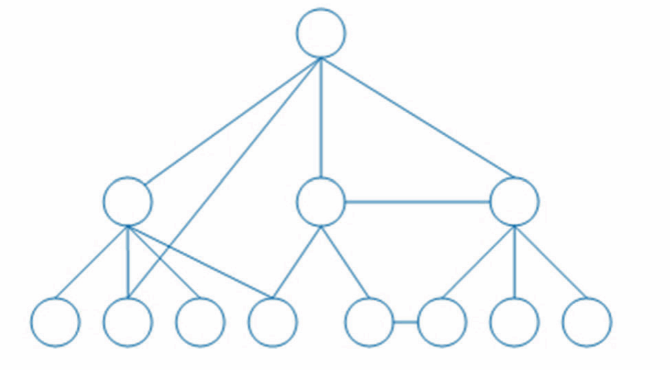
\includegraphics[height=0.25\textheight]{img/setevoy.png}
	\caption{Cхема сетевой модели \cite{roders}}
	\label{img:setevoy}
\end{figure}

\subsubsection{Реляционные}
Реляционная модель данных включает в себя следующие компоненты:
\begin{itemize}
	\item структурный компонент --- данные организованы в базе данных в виде набора отношений, представленных в виде таблиц;
	\item целостностный компонент --- отношения (или таблицы) в базе данных должны соответствовать определенным условиям целостности, чтобы гарантировать правильность и непротиворечивость данных.
	\item манипуляционный компонент --- для выполнения операций над данными используются средства реляционной алгебры и реляционного исчисления.
\end{itemize}
\subsubsection{Постреляционные}
Это расширенная версия реляционной модели, которая позволяет хранить множественные значения в полях данных и разделять их на подзначения. Однако, сложность обеспечения целостности данных является ее главным недостатком.

На рисунке \ref{img:relation} приведены реляционная и постреляционная модели данных для одной и той же предметной области.

\begin{figure}[h]
	\centering
	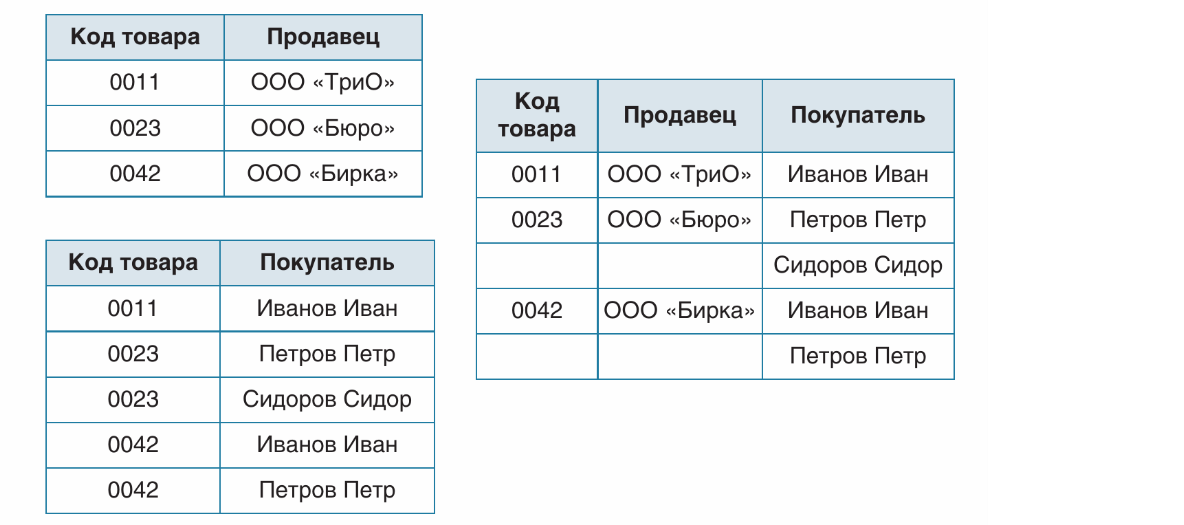
\includegraphics[height=0.25\textheight]{img/relation.png}
	\caption{Реляционная (слева) и постреляционная (справа) модели данных \cite{roders}}
	\label{img:relation}
\end{figure}

\subsubsection{Выбор модели организации данных}
Поскольку задача требует выполнения разнообразных запросов, которые включают в себя сложные операции выборки данных по разным критериям, наиболее важными качествами модели данных являются гибкость, простота использования, целостность данных и независимость от приложения.
Именно поэтому реляционная модель организации данных была выбрана.

\subsection{Формализация данных}

Выделяются следующие сущности, которые в базе данных должны хранить:
\begin{itemize}
	\item пользователь;
	\item турнир;
	\item команда
	\item стадион;
	\item страна;
	\item матч;
	\item отзыв;
	\item заявка.
\end{itemize}

Информация о каждой сущности проводится в таблице~\ref{tb:data}.

\begin{table}[ht]
	\begin{center}
		\begin{threeparttable}
			\caption{\label{tb:data} Сущности и их описания}
			\begin{tabular}{|c|p{10cm}|}
				\hline
				\textbf{Сущность} & \textbf{Описание} \\ \hline
				Пользователь & Логин, пароль, роль, фамилия, имя, возраст, команда \\ \hline
				Турнир & Название, рейтинг, страна, создатель \\ \hline
				Стадион & Название, количество мест, страна \\ \hline
				Страна & Название, континент \\ \hline
				Команда & Название, страна \\ \hline
				Заявка & Время создания, создатель, команда, турнир \\ \hline
				Матч & Готевая команда, домашняя команда, голы гостевой, голы домашнней, турнир, стадион, неделя, время проведения \\ \hline
				Отзыв & Пользователь, оценка, турнир \\ \hline
			\end{tabular}
		\end{threeparttable}
	\end{center}
\end{table}

\newpage

На рисунке \ref{img:ER} приведена ER-диаграмма сущностей в нотации Чена.

\begin{figure}[h]
	\centering
	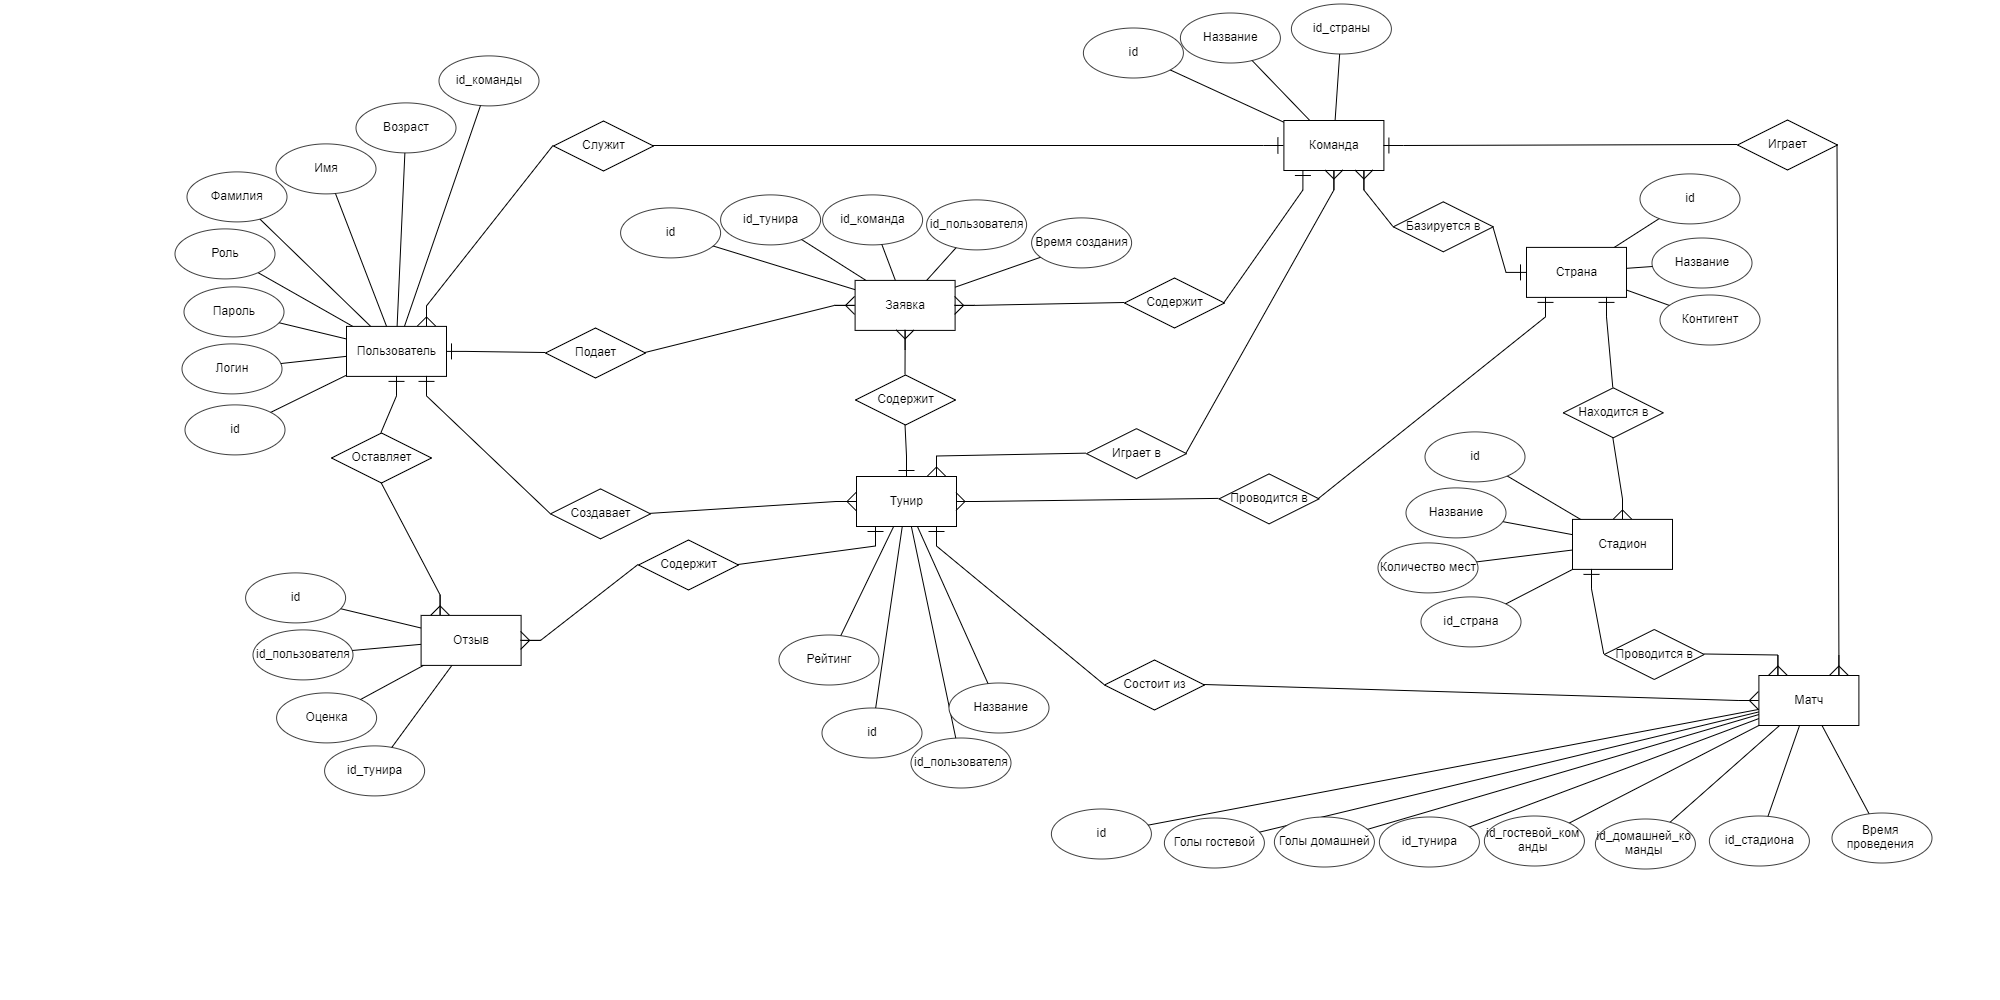
\includegraphics[height=0.3\textheight]{img/ER.png}
	\caption{ER-диаграмма сущностей}
	\label{img:ER}
\end{figure}
\subsection{Системные пользователи}

В приложении выделяются пять видов ролей:
\begin{enumerate}
	\item Гость --- неавторизованный пользователь, который обладающий возможностями зарегистрировать, входить в систему, просмотреть расписания турниров, посмотреть  статистики турниров, оставить свои отзывы.
	\item Футболист --- авторизованный пользователь, который может подать заявку на поступление в клуб, просмотреть все информации о турнирах.
	\item Тренер --- авторизованный пользователь, который может создать свой клуб, принять/отменить заявку футболистов, подать заявку на поступление в турнир, просмотреть все информации о турнирах.
	\item Судья --- авторизованный пользователь, который может создать свои турниры, принять/отменить заявку тренеров, составить расписания турниров, вводить результаты матча.
	\item Администатор --- пользователь, обладающий возможностями всех вышеперечисленных пользователей. Кроме этого, он может изменять данных пользователей и турниров.
\end{enumerate}

На рисунках \ref{img:Use-case1}--\ref{img:Use-case2} приведена Use-Case диаграмма.

\begin{figure}[h]
	\centering
	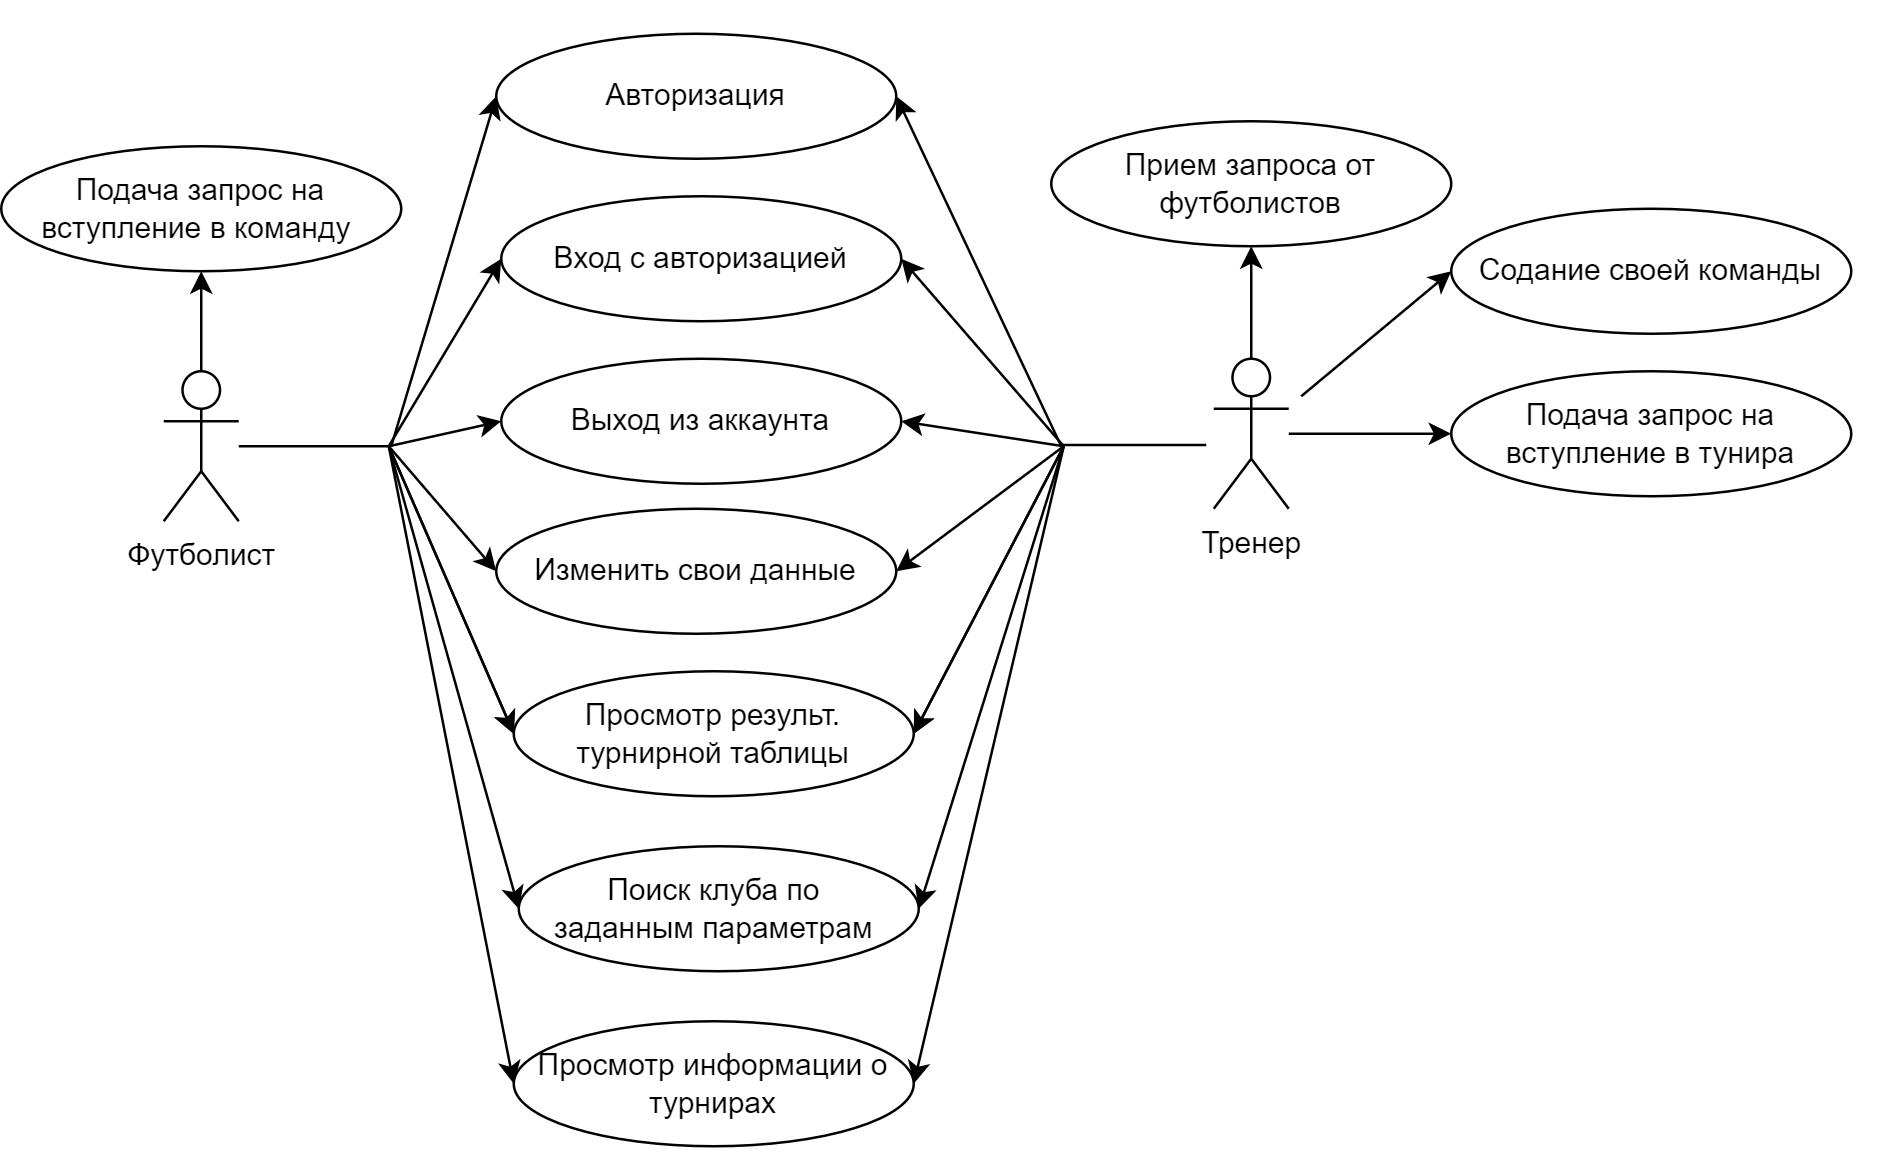
\includegraphics[height=0.3\textheight]{img/ppo-Use-Case1.png}
	\caption{Use-Case диаграмма}
	\label{img:Use-case1}
\end{figure}

\begin{figure}[h]
	\centering
	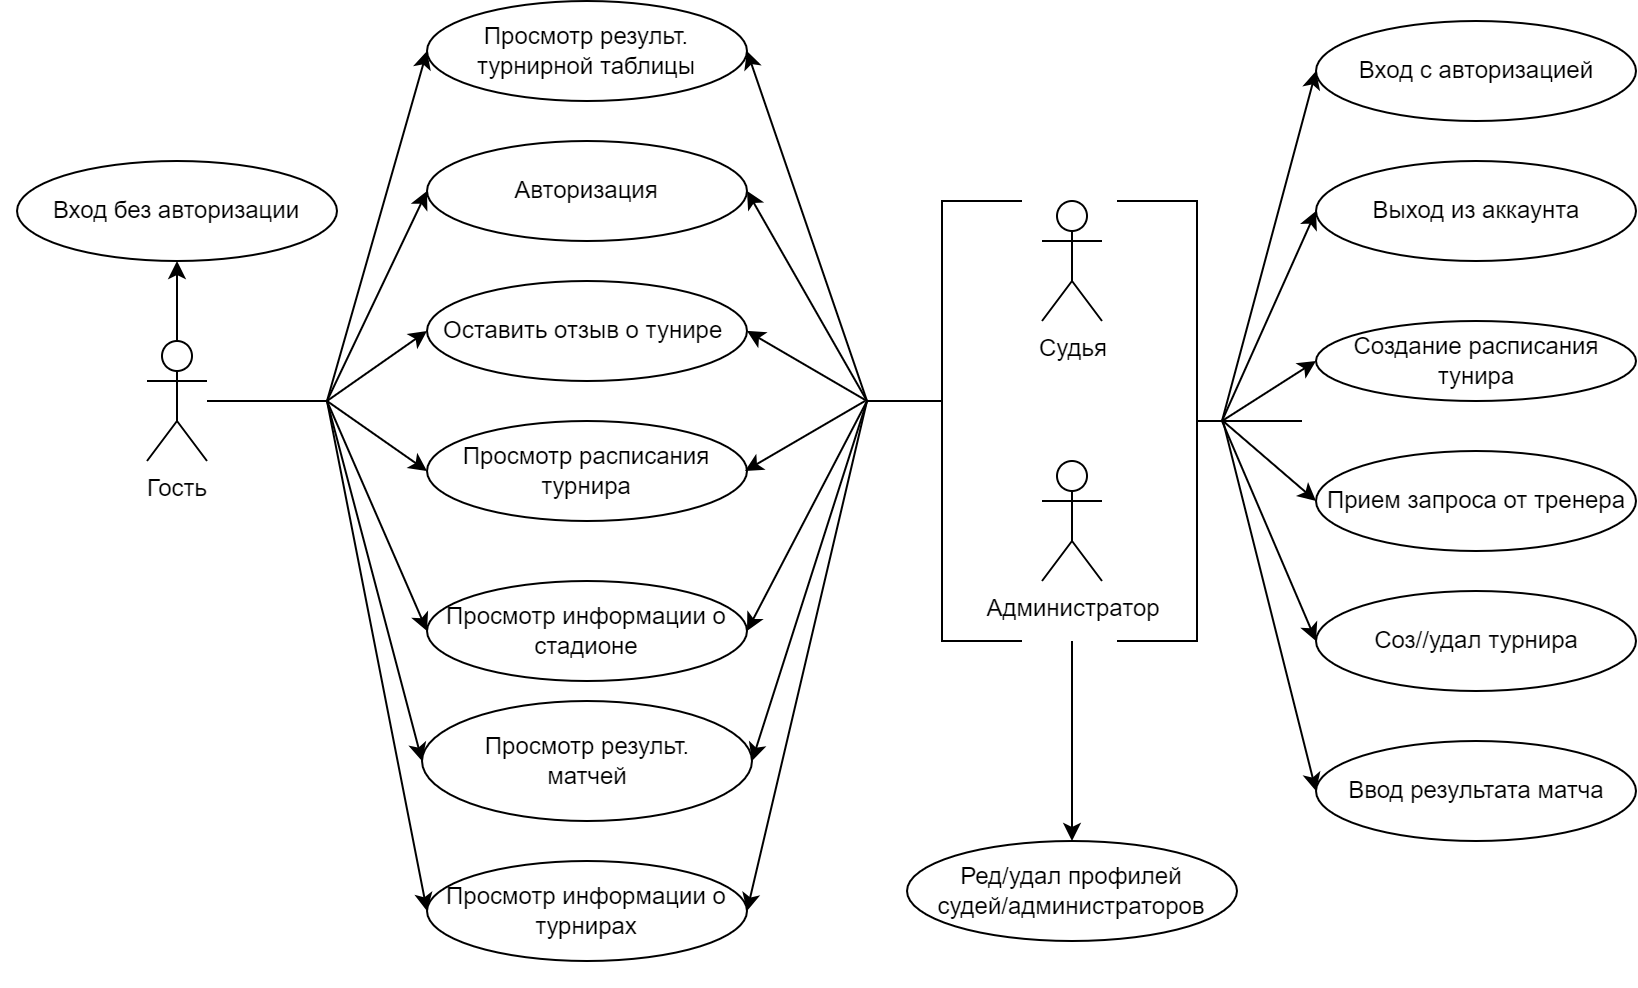
\includegraphics[height=0.3\textheight]{img/ppo-Use-Case2.png}
	\caption{Use-Case диаграмма (продолжение)}
	\label{img:Use-case2}
\end{figure}

\clearpage

\subsection*{Вывод}
В данном разделе была проанализирована предметная область.
Была преведена постановка задачи, формализация данных и построена соотвествующая ER-диаграмма. 
Также описаны системные пользователи.
Проведен анализ баз данных по модели данных и на основе этого анализа была выбрана подходящая модель для решения поставленной задачи.